%!TEX TS-program = xelatex
%!TEX encoding = UTF-8 Unicode

\documentclass[12pt]{extarticle}
% extarticle is like article but can handle 8pt, 9pt, 10pt, 11pt, 12pt, 14pt, 17pt, and 20pt text

\def \ititle {Philosophical Psychology}

\def \isubtitle {Lecture 08}

\def \iauthor {Stephen A. Butterfill}
\def \iemail{s.butterfill@warwick.ac.uk}
\date{}

%for strikethrough
\usepackage[normalem]{ulem}

\input{$HOME/latex_imports/preamble_steve_handout}

%\bibpunct{}{}{,}{s}{}{,}  %use superscript TICS style bib
%remove hanging indent for TICS style bib
%TODO doesnt work
\setlength{\bibhang}{0em}
%\setlength{\bibsep}{0.5em}


%itemize bullet should be dash
\renewcommand{\labelitemi}{$-$}

\begin{document}

\begin{multicols*}{3}

\setlength\footnotesep{1em}


\bibliographystyle{newapa} %apalike

%\maketitle
%\tableofcontents




%---------------
%--- start paste




\def \ititle {08: A Dual-Process Theory of Mindreading}

\begin{center}

{\Large

\textbf{\ititle}

}



\iemail %

\end{center}

\begin{center}
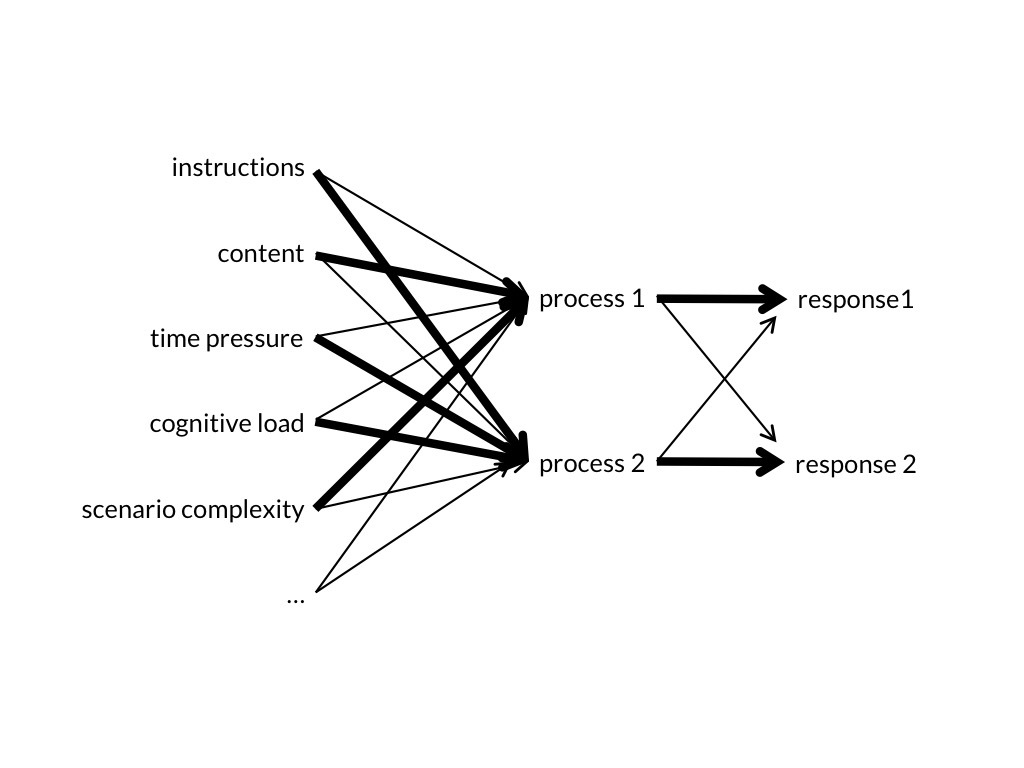
\includegraphics[scale=0.3]{img/dual_process_operationalized_11.neg.jpg}
\end{center}

\emph{Dual Process Theory (core part)}:
Two (or more) processes for tracking Xs are distinct:
the conditions which influence whether they occur,
and which outputs they generate,
do not completely overlap.

%--- end paste
%---------------

\footnotesize
% \bibliography{$HOME/endnote/phd_biblio}

\end{multicols*}

\end{document}
